\documentclass[11pt]{article}

\usepackage[a4paper,top=1in,bottom=1in,left=0.75in,right=0.75in]{geometry}
\usepackage{amsmath,amssymb}
\usepackage{array,booktabs,longtable,tabularx}
\usepackage{graphicx}
\usepackage{xcolor}
\usepackage{microtype}

\setlength{\parindent}{0pt}
\setlength{\parskip}{0.35em}
\renewcommand{\arraystretch}{1.16}
\newcolumntype{L}[1]{>{\raggedright\arraybackslash}p{#1}}
\newcolumntype{C}[1]{>{\centering\arraybackslash}p{#1}}
\newcolumntype{Y}{>{\centering\arraybackslash}l}
\newcolumntype{Z}{>{\raggedright\arraybackslash}X}
\newcolumntype{M}{>{\centering\arraybackslash}X}
\newcolumntype{R}[1]{>{\raggedleft\arraybackslash}p{#1}}

\begin{document}


\section*{Appendix A: BSA-D2 Hardware and Actuator Settings}

\begin{center}
\footnotesize
\begin{tabularx}{\textwidth}{@{}Z M M@{}}
\toprule
Parameter & Value & Unit \\
\midrule
BSA-D2 mass & 19.450606146 & kg \\
COM $x$ & 0.048901198 & m \\
COM $y$ & 0.020260562 & m \\
COM $z$ & 0.048221021 & m \\
Inertia $J_{xx}$ & 0.193749459 & $\mathrm{kg}\cdot\mathrm{m}^2$ \\
Inertia $J_{xy}$ & 0.017485528 & $\mathrm{kg}\cdot\mathrm{m}^2$ \\
Inertia $J_{xz}$ & 0.033545050 & $\mathrm{kg}\cdot\mathrm{m}^2$ \\
Inertia $J_{yy}$ & 1.847824640 & $\mathrm{kg}\cdot\mathrm{m}^2$ \\
Inertia $J_{yz}$ & 0.006924042 & $\mathrm{kg}\cdot\mathrm{m}^2$ \\
Inertia $J_{zz}$ & 1.895445823 & $\mathrm{kg}\cdot\mathrm{m}^2$ \\
Action dimension & 5 & -- \\
Action lower bound & $-1$ & -- \\
Action upper bound & $1$ & -- \\
Forward-force scale & $-90$ & N \\
Lateral-force scale & $-60$ & N \\
Vertical-force scale & 45 & N \\
Pitch-torque scale & 18 & $\mathrm{N}\cdot\mathrm{m}$ \\
Yaw-torque scale & 18 & $\mathrm{N}\cdot\mathrm{m}$ \\
Roll PD $k_p$ & 6.0 & -- \\
Roll PD $k_d$ & 3.0 & -- \\
Roll torque limit & 8.0 & $\mathrm{N}\cdot\mathrm{m}$ \\
Allocation force fraction & 0.50 & -- \\
Allocation warning threshold & $10^{-3}$ & -- \\
Vehicle thruster reverse limit & $-30.69$ & N \\
Vehicle thruster forward limit & 37.56 & N \\
PWM neutral value & 1500 & $\mu$s \\
\bottomrule
\end{tabularx}
\end{center}

\begin{center}
\footnotesize
\setlength{\tabcolsep}{2.5pt}
\begin{tabular*}{\textwidth}{@{\extracolsep{\fill}}L{0.20\textwidth}*{8}{C{0.075\textwidth}}@{}}
\toprule
Thruster & $P_1$ & $P_2$ & $P_3$ & $P_4$ & $P_5$ & $P_6$ & $P_7$ & $P_8$ \\
\midrule
Mounting & aft & aft & aft & fore & aft & fore & fore & fore \\
Type & vectored & vectored & vertical & vertical & vertical & vertical & vectored & vectored \\
$F_x$ & $-1/\sqrt{2}$ & $-1/\sqrt{2}$ & 0 & 0 & 0 & 0 & $+1/\sqrt{2}$ & $+1/\sqrt{2}$ \\
$F_y$ & $+1/\sqrt{2}$ & $-1/\sqrt{2}$ & 0 & 0 & 0 & 0 & $+1/\sqrt{2}$ & $-1/\sqrt{2}$ \\
$F_z$ (up $+$) & 0 & 0 & $+1$ & $+1$ & $+1$ & $+1$ & 0 & 0 \\
\bottomrule
\end{tabular*}
\par\vspace{2pt}
\parbox{\textwidth}{\scriptsize\raggedright
Eight TS60 thrusters (Fig.~1(d) of the main text): four vectored horizontal units at the corners ($\pm45^{\circ}$; $P_1$, $P_2$ aft; $P_7$, $P_8$ fore) and four vertical units ($P_3$, $P_5$ aft; $P_4$, $P_6$ fore). Normalized force directions under positive commands; $F_y>0$ toward starboard. Roll, pitch, and yaw moments are generated differentially by the port--starboard and fore--aft vertical pairs and by opposing vectored thrusters.
}
\end{center}

\clearpage
\section*{Appendix B: Isaac Sim Simulation Parameters}

\begin{center}
\footnotesize
\begin{tabularx}{\textwidth}{@{}Z M M Z@{}}
\toprule
Parameter & Value & Unit & Source/Use \\
\midrule
Physics rate & 50 & Hz & PhysX \\
Policy rate & 10 & Hz & SAC \\
Decimation & 5 & -- & PhysX/SAC \\
Mass randomization range & $[16,22]$ & kg & random. \\
Inertia-scale randomization range & $[0.60,1.60]$ & -- & random. \\
Pool-policy mass/inertia scale & $\mathcal{U}(0.8,1.2)$ & -- & pool train \\
Pool-policy damping scale & $\times[0.7,1.3]$ (lin./ang., indep.) & -- & pool train \\
Pool-policy training steps & $10^6$ (with/without randomization) & -- & pool train \\
Linear damping $D_1$ & $\mathrm{diag}(8.0,8.0,6.0)$ & -- & drag \\
Quadratic damping $D_2$ & $\mathrm{diag}(4.0,4.0,3.0)$ & -- & drag \\
Training current speeds & $\{0.1,0.3,0.5\}$ & m/s & train \\
Evaluation current speeds & $\{0.0,0.1,0.3,0.5\}$ & m/s & eval. \\
Training current direction & $+90^{\circ}$ (still water included) & -- & train \\
Held-out current direction & $-90^{\circ}$ (excluded from training) & -- & eval. \\
Evaluation conditions & training $\cup$ held-out, 42 configurations & -- & eval. \\
RGB preview camera & $640\times360$ & pixels & figures only \\
Depth camera & Ray-cast range camera & -- & depth \\
Depth image width & 80 & pixels & depth \\
Depth image height & 45 & pixels & depth \\
Horizontal field of view & 110.0 & deg & depth \\
Vertical field of view & 70.0 & deg & depth \\
Maximum range & 60.0 & m & depth \\
Depth encoding & $\log(1+d)/\log(61)$ & -- & depth \\
Depth history length & 4 & frames & visual \\
Depth frame interval & 0.1 (one per control step) & s & visual \\
Minimum valid depth & 0.25 & m & depth \\
Sector depth quantile & 0.05 & -- & clearance \\
Minimum valid-pixel ratio & 0.30 & -- & depth \\
Visual observation dimension & 31 & -- & obs. \\
\bottomrule
\end{tabularx}
\end{center}


\clearpage
\section*{Appendix C: CSPI-LLM Component and Network Architecture}

\begin{center}
\scriptsize
\begin{tabularx}{\textwidth}{@{}Z Z Z@{}}
\toprule
Item & Value & Use \\
\midrule
Teacher window & $(t-1.5,t-1.0,t-0.5,t)$ & 4-frame window \\
Window rate & 2 Hz & from 10 Hz trajectory, stride 5 \\
Allowed inputs & body/DVL velocity, IMU angular rate, body-frame goal direction, goal-distance trend, directional clearances, previous action, Fossen-lite proxy & deployable observation \\
Excluded inputs & route ID, true current, relative-water truth, waypoint/cross-track oracle, oracle progress, reward terms & no privileged input \\
Lateral drift proxy & $d_{y,t}=\widehat v_t-0.25a_{F_y,t-1}$ & Fossen-lite \\
Vertical drift proxy & $d_{z,t}=\widehat w_t-0.25a_{F_z,t-1}$ & Fossen-lite \\
Drag proxy & $d_{D,t}=\left\|{}^b\widehat{\mathbf v}_t\odot\left|{}^b\widehat{\mathbf v}_t\right|\right\|_2$ & Fossen-lite \\
Braking-demand proxy & $d_{\mathrm{brake},t}=\max(\hat u_t,0)^2/(2a_{\mathrm{dec}}^{\mathrm{cons}})$ & Fossen-lite \\
Progress-loss proxy & $d_{\mathrm{loss},t}=\max(0,p_{\mathrm{expected},t}-p_{\mathrm{observed},t})$ & Fossen-lite \\
Clearance margin & $d_i-d_{\mathrm{safe},i}$ & safety evidence \\
$a_{\mathrm{dec}}^{\mathrm{cons}}$ & $0.50~\mathrm{m/s^2}$ & safety-distance/barrier \\
Safety thresholds & front $12.0~\mathrm{m}$, side $8.0~\mathrm{m}$, vertical $8.0~\mathrm{m}$ & Fossen-lite \\
Bin thresholds & lateral $1.50~\mathrm{m/s}$, vertical $1.30~\mathrm{m/s}$, progress-loss $0.30~\mathrm{m/s}$, drag $2.25~\mathrm{m^2/s^2}$ & qualitative evidence \\
Output schema & 8 yes/no keys & teacher target \\
Reserved ninth field & STOP\_HOLD = 0 & semantic vector \\
Final filtering & $48{,}599\rightarrow48{,}587$ & SFT dataset \\
Removed samples & empty 4, left-right conflict 4, up-down conflict 4 & filtering \\
Semantic executability & left/right and up/down are mutually exclusive & not formal reachability \\
Online safety fusion & front\_critical 0.08, front\_low 0.16, side\_critical 0.08, side\_low 0.14, reverse\_critical 0.04, direction\_margin 0.08 & semantic label correction \\
Pool safety fusion & front\_critical 0.28, front\_low 0.35, side\_critical 0.18, side\_low 0.22, reverse\_critical 0.12, direction\_margin 0.08 & onboard trials \\
Safety-fusion scope & modifies semantic labels only; does not overwrite SAC action & online fallback \\
\bottomrule
\end{tabularx}
\end{center}

\begin{center}
\footnotesize
\begin{tabular*}{\textwidth}{@{\extracolsep{\fill}}L{0.34\textwidth}L{0.38\textwidth}L{0.20\textwidth}@{}}
\toprule
Component & Parameter & Value \\
\midrule
LLM checkpoint & Local recovered backbone & Qwen3-4B-Instruction \\
LLM text stack & Hidden layers & 36 \\
LLM text stack & Hidden size & 2560 \\
LLM text stack & Attention heads & 32 \\
LLM text stack & Key-value heads & 8 \\
LLM text stack & Intermediate size & 9728 \\
LLM text stack & Maximum positions & 40960 \\
LLM text stack & Vocabulary size & 151936 \\
Semantic output head & Multilabel semantic vector & 9 labels \\
GateNet input & Semantic vector plus hold age & 10 values \\
Visual branch & Four-frame depth history embedding ($4\times45\times80$, single channel) & $d_v=128$ \\
Visual stream Transformer & Layers & 2 \\
Visual stream Transformer & Attention heads & 4 \\
Visual stream Transformer & $d_{\mathrm{model}}$ & 128 \\
Navigation branch & Deployable navigation embedding & $d_n=64$ \\
Navigation stream Transformer & Layers & 2 \\
Navigation stream Transformer & Attention heads & 4 \\
Navigation stream Transformer & $d_{\mathrm{model}}$ & 64 \\
Feature fusion & Fused feature dimension & $d_f=256$ \\
Fusion encoder & Layers & 2 \\
Fusion encoder & Attention heads & 4 \\
Fusion encoder & $d_{\mathrm{model}}$ & 256 \\
Policy input & State dimension & 38 values (28 + 9 + 1) \\
Actor head & Action dimension & 5 \\
Actor distribution & Squashed Gaussian policy & enabled \\
Actor log-std range & Lower / upper bounds & $[-5,1]$ \\
Critic heads & Twin Q critics & 2 critics \\
\bottomrule
\end{tabular*}
\end{center}

\vspace{4pt}
\noindent\textbf{Perception inputs by module.} No module consumes color images. The features extracted by the SAC encoders are used only by the actor and critics; the language teacher and student receive numeric text only.

\begin{center}
\footnotesize
\begin{tabular*}{\textwidth}{@{\extracolsep{\fill}}L{0.23\textwidth}L{0.37\textwidth}L{0.14\textwidth}L{0.18\textwidth}@{}}
\toprule
Consumer & Input & Size & Rate \\
\midrule
SAC visual stream & Depth stack, single channel & $4\times45\times80$ & 10 Hz \\
SAC navigation stream & Deployable navigation vector & 28 & 10 Hz \\
GateNet & Safety-fused semantic vector, normalized commit age & $9+1$ & 2-Hz requests; age at 10 Hz \\
Language teacher and student & Numeric observation summary and Fossen-lite evidence (text) & 31-D summary $+$ proxies & 2-Hz four-frame window \\
SAC actor and critics & Fused, gated features & 256 & 10 Hz \\
\bottomrule
\end{tabular*}
\end{center}

\noindent\begin{minipage}{\textwidth}
\textbf{Numeric policy input.} The non-visual part of $\mathbf x_t$ in (5) of the main text is a 38-D vector with the following fixed layout.

\begin{center}
\footnotesize
\begin{tabular*}{\textwidth}{@{\extracolsep{\fill}}L{0.10\textwidth}L{0.32\textwidth}L{0.10\textwidth}L{0.40\textwidth}@{}}
\toprule
Index & Entry & Dim. & Normalization \\
\midrule
0--2 & DVL body velocity & 3 & scaled, clipped to $[-1,1]$ \\
3--6 & DVL beam ranges & 4 & $\log(1+r)/\log(1+r_{\max})$, clipped to $[0,1]$ \\
7--10 & DVL beam hit flags & 4 & binary \\
11--14 & Attitude quaternion & 4 & unit norm, sign-canonical \\
15--17 & Angular rate & 3 & scaled, clipped to $[-1,1]$ \\
18 & Pressure depth & 1 & centered, scaled, clipped to $[-1,1]$ \\
19--21 & Goal direction & 3 & unit vector \\
22 & Goal distance & 1 & scaled, clipped to $[0,1]$ \\
23--27 & Previous action & 5 & $[-1,1]$ \\
\midrule
\multicolumn{2}{@{}l}{Navigation subtotal} & 28 & \\
\midrule
28--36 & Safety-fused semantic vector $\mathbf m_t^{\mathrm{safe}}$ & 9 & binary \\
37 & Normalized commit age $\overline{\Delta t}_t^{\mathrm{sem}}$ & 1 & $\min\{1,\Delta t_k^{\mathrm{sem}}/\Delta t_{\max}\}$ \\
\midrule
\multicolumn{2}{@{}l}{Total} & 38 & \\
\bottomrule
\end{tabular*}
\end{center}
\end{minipage}

\noindent\textbf{Privileged expert input.} The privileged expert used as the upper reference in Table~II of the main text receives the same 28-D navigation block followed by 19 privileged entries: true current velocity in the body frame (3), next waypoint (3), path tangent (3), cross-track error (1), progress along the planned path (1), distance to the next waypoint (1), current planned clearance (1), minimum planned clearance ahead (1), and five sector clearances (5); its numeric state is therefore 47-D. These entries are never supplied to CSPI-LLM.

\clearpage
\section*{Appendix D: LLM and DRL Training Hyperparameters}

\begin{center}
\footnotesize
\begin{tabularx}{\textwidth}{@{}Z M M Z@{}}
\toprule
Parameter & Value & Unit & Source/Use \\
\midrule
Filtered semantic samples & 48587 & samples & LLM train \\
LoRA rank $r_L$ & 8 & -- & LLM train \\
LoRA scale $\alpha_L$ & 16 & -- & LLM train \\
LoRA dropout & 0.05 & -- & LLM train \\
LLM learning rate & $1.5\times10^{-5}$ & -- & LLM train \\
Warmup ratio & 0.05 & -- & LLM train \\
Per-device batch & 8 & samples & LLM train \\
Gradient accumulation & 2 & steps & LLM train \\
Effective batch & 16 & samples & LLM train \\
LLM epochs & 2.0 & epochs & LLM train \\
Sequence length & 1024 & tokens & LLM train \\
Validation split & 0.05 & -- & LLM train \\
Evaluation batch & 8 & samples & LLM train \\
$\gamma_{\mathrm{SAC}}$ & 0.995 & -- & SAC train \\
SAC learning rate & $3.0\times10^{-4}$ & -- & SAC train \\
Target smoothing $\tau$ & 0.005 & -- & SAC train \\
Replay buffer size & 300000 & transitions & SAC train \\
Learning start & 50000 & transitions & SAC train \\
SAC batch size & 512 & samples & SAC train \\
Train frequency & 1 & step & SAC train \\
Gradient steps & 1 & step & SAC train \\
Entropy coefficient & auto\_0.05 & -- & SAC train \\
Target entropy & $-5.0$ & -- & SAC train \\
Target update interval & 1 & step & SAC train \\
Optimizer epsilon & $10^{-5}$ & -- & SAC train \\
\bottomrule
\end{tabularx}
\end{center}

\clearpage
\section*{Appendix D (continued): Reward and Training Objectives}
\setcounter{equation}{0}
\renewcommand{\theequation}{D.\arabic{equation}}

The terminal reward replaces the nonterminal progress, time, action-magnitude, and action-variation reward on terminal transitions:
\begin{equation}
r_t^{\mathrm{term}}
=
\begin{cases}
+300, & \mathrm{success},\\
-300, & \mathrm{contact},\\
-300, & \mathrm{out\ of\ bounds},\\
-100, & \mathrm{timeout},\\
0, & \mathrm{otherwise}.
\end{cases}
\label{eq:terminal_reward}
\end{equation}

The nonterminal weights are $w_d=8.0$, $w_t=-0.05$, $w_a=0.01$, and $w_{\Delta a}=0.005$, with initial previous action $\mathbf a_{-1}=\mathbf0$. The safe-distance progress field is unavailable to the actor and both language models.

For a frozen weight matrix $\mathbf W_0$, an adapted layer is
\begin{equation}
\mathbf{h}
=
\mathbf{W}_0\mathbf{x}
+
\frac{\alpha_{\mathrm{L}}}{r_{\mathrm{L}}}
\mathbf{B}\mathbf{A}\mathbf{x},
\label{eq:lora}
\end{equation}
where $\mathbf{x}$ and $\mathbf{h}$ denote the layer input and output, $\mathbf{A}$ and $\mathbf{B}$ are the trainable low-rank factors, and $r_{\mathrm{L}}$ and $\alpha_{\mathrm{L}}$ are the LoRA rank and scale. Rank, scale, and dropout are listed in the preceding hyperparameter table.

The actor and critic interfaces are defined in Section~III-D of the main text. Here, $\widetilde{\mathbf z}_t^\pi$ and $\widetilde{\mathbf z}_t^{Q_i}$ denote their independently gated features, while $\theta$ and $\phi_i$ parameterize the actor and the $i$th critic.

The SAC target is
\begin{equation}
\begin{aligned}
y_t
={}&
r_t+\gamma_{\mathrm{RL}}(1-d_t)
\big[
\min_i
Q_{\bar\phi_i}
(\widetilde{\mathbf{z}}_{t+1}^{Q_i},\mathbf{a}_{t+1})\\
&\hspace{6em}
-\alpha
\log
\pi_{\theta}
(\mathbf{a}_{t+1}
\mid
\widetilde{\mathbf{z}}_{t+1}^{\pi})
\big],
\end{aligned}
\label{eq:sac_target}
\end{equation}
where $d_t$ is the terminal indicator, $\alpha$ is the entropy coefficient, and $\bar\phi_i$ denotes the target-critic parameters. The critic and actor objectives are
\begin{equation}
\begin{aligned}
J_Q(\phi_i)
&=
\mathbb{E}
\left[
\left(
Q_{\phi_i}
(\widetilde{\mathbf{z}}_t^{Q_i},\mathbf{a}_t)
-y_t
\right)^2
\right],\\
J_{\pi}(\theta)
={}&
\mathbb{E}\Bigl[
\alpha
\log
\pi_{\theta}
(\mathbf{a}_t\mid\widetilde{\mathbf{z}}_t^{\pi})
-
\min_i
Q_{\phi_i}
(\widetilde{\mathbf{z}}_t^{Q_i},\mathbf{a}_t)
\Bigr].
\end{aligned}
\label{eq:sac_objectives}
\end{equation}
The target and objectives retain the standard SAC formulation. Semantic conditioning is supplied through the independently gated actor and critic features defined in the main text.

\clearpage
\section*{Appendix E: LLM Internal Component Comparison}

\begin{center}
\scriptsize
\begin{tabular*}{\textwidth}{@{\extracolsep{\fill}}L{0.30\textwidth}L{0.19\textwidth}L{0.19\textwidth}L{0.19\textwidth}@{}}
\toprule
Component / field & Qwen3-0.6B & Qwen3-4B-Instruction & Qwen3-8B \\
\midrule
Family & Qwen3 & Qwen3 & Qwen3 \\
Model class & Qwen3ForCausalLM & Qwen3ForCausalLM & Qwen3ForCausalLM \\
Model type & qwen3 & qwen3 & qwen3 \\
Parameter scale & 0.6B & 4B & 8B \\
Architecture type & decoder-only causal LM & decoder-only causal LM & decoder-only causal LM \\
Hidden size & 1024 & 2560 & 4096 \\
Decoder layers & 28 & 36 & 36 \\
Attention heads & 16 & 32 & 32 \\
Key-value heads & 8 & 8 & 8 \\
Head dimension & 128 & 128 & 128 \\
Attention projection width & 2048 & 4096 & 4096 \\
Query heads per KV head & 2 & 4 & 4 \\
GQA setting & grouped-query attention & grouped-query attention & grouped-query attention \\
MLP intermediate size & 3072 & 9728 & 12288 \\
FFN expansion ratio & 3.00 & 3.80 & 3.00 \\
Activation & SiLU & SiLU & SiLU \\
Vocabulary size & 151936 & 151936 & 151936 \\
Token embedding shape & $151936\times1024$ & $151936\times2560$ & $151936\times4096$ \\
Embedding parameters & 155.6M & 389.0M & 622.3M \\
Output embedding tying & tied & tied & untied \\
Maximum positions & 40960 & 40960 & 40960 \\
Maximum window layers & 28 & 36 & 36 \\
Sliding-window size & null & null & null \\
Use sliding window & false & false & false \\
RMSNorm epsilon & $10^{-6}$ & $10^{-6}$ & $10^{-6}$ \\
RoPE theta & 1000000 & 1000000 & 1000000 \\
RoPE scaling & null & null & null \\
Initializer range & 0.02 & 0.02 & 0.02 \\
Attention bias & false & false & false \\
Attention dropout & 0.0 & 0.0 & 0.0 \\
Input BOS token ID & 151643 & 151643 & 151643 \\
Output EOS token ID & 151645 & 151645 & 151645 \\
Torch dtype & bfloat16 & bfloat16 & bfloat16 \\
Use cache & true & true & true \\
Transformers version & 4.51.0 & 4.51.0 & 4.51.0 \\
\bottomrule
\end{tabular*}
\end{center}

\clearpage
\section*{Appendix F: DRL Training Summary}

\begin{center}
\scriptsize
\setlength{\tabcolsep}{3pt}
\begin{tabular*}{\textwidth}{@{\extracolsep{\fill}}L{0.22\textwidth}*{5}{C{0.115\textwidth}}@{}}
\toprule
Hyperparameter & CSPI-LLM / SAC & SAC & TD3 & DDPG & TQC \\
\midrule
Learning rate & $3\times10^{-4}$ & $3\times10^{-4}$ & $3\times10^{-4}$ & $3\times10^{-4}$ & $3\times10^{-4}$ \\
Discount gamma & 0.995 & 0.995 & 0.99 & 0.99 & 0.99 \\
Replay buffer & 300,000 & 300,000 & 300,000 & 300,000 & 300,000 \\
Batch size & 512 & 512 & 256 & 256 & 256 \\
Learning starts & 50,000 & 50,000 & 50,000 & 50,000 & 50,000 \\
Target smoothing tau & 0.005 & 0.005 & 0.005 & 0.005 & 0.005 \\
Entropy coefficient & auto\_0.05 & auto\_0.05 & -- & -- & auto \\
Target entropy & $-5.0$ & $-5.0$ & -- & -- & auto \\
Policy delay & -- & -- & 2 & -- & -- \\
Target policy noise & -- & -- & 0.2 & -- & -- \\
Target noise clip & -- & -- & 0.5 & -- & -- \\
Action noise std. & -- & -- & 0.15 & 0.20 & 0.15 \\
Dropped quantiles & -- & -- & -- & -- & 2 \\
Batch norm & -- & -- & -- & -- & -- \\
Parallel environments & 32 & -- & -- & -- & -- \\
Semantic interface & enabled & disabled & disabled & disabled & disabled \\
\bottomrule
\end{tabular*}
\end{center}

\begin{center}
\scriptsize
\setlength{\tabcolsep}{3pt}
\begin{tabular*}{\textwidth}{@{\extracolsep{\fill}}L{0.22\textwidth}*{3}{C{0.14\textwidth}}@{}}
\toprule
Hyperparameter & PPO & TRPO & Recurrent PPO \\
\midrule
Learning rate & $3\times10^{-4}$ & $3\times10^{-4}$ & $3\times10^{-4}$ \\
Discount gamma & 0.99 & 0.99 & 0.99 \\
Rollout steps & 512 & 512 & 256 \\
Batch size & 2,048 & 2,048 & 1,024 \\
Epochs & 5 & -- & 5 \\
GAE lambda & 0.95 & 0.95 & 0.95 \\
Clip range & 0.2 & -- & 0.2 \\
Entropy coefficient & 0.01 & -- & 0.01 \\
Value loss coefficient & 0.5 & -- & 0.5 \\
Max grad norm & 0.5 & -- & 0.5 \\
TRPO target KL & -- & 0.01 & -- \\
TRPO CG steps & -- & 15 & -- \\
LSTM hidden & -- & -- & 256 \\
LSTM layers & -- & -- & 1 \\
\bottomrule
\end{tabular*}
\end{center}

\clearpage
\section*{Appendix G: Fig. 1}

\noindent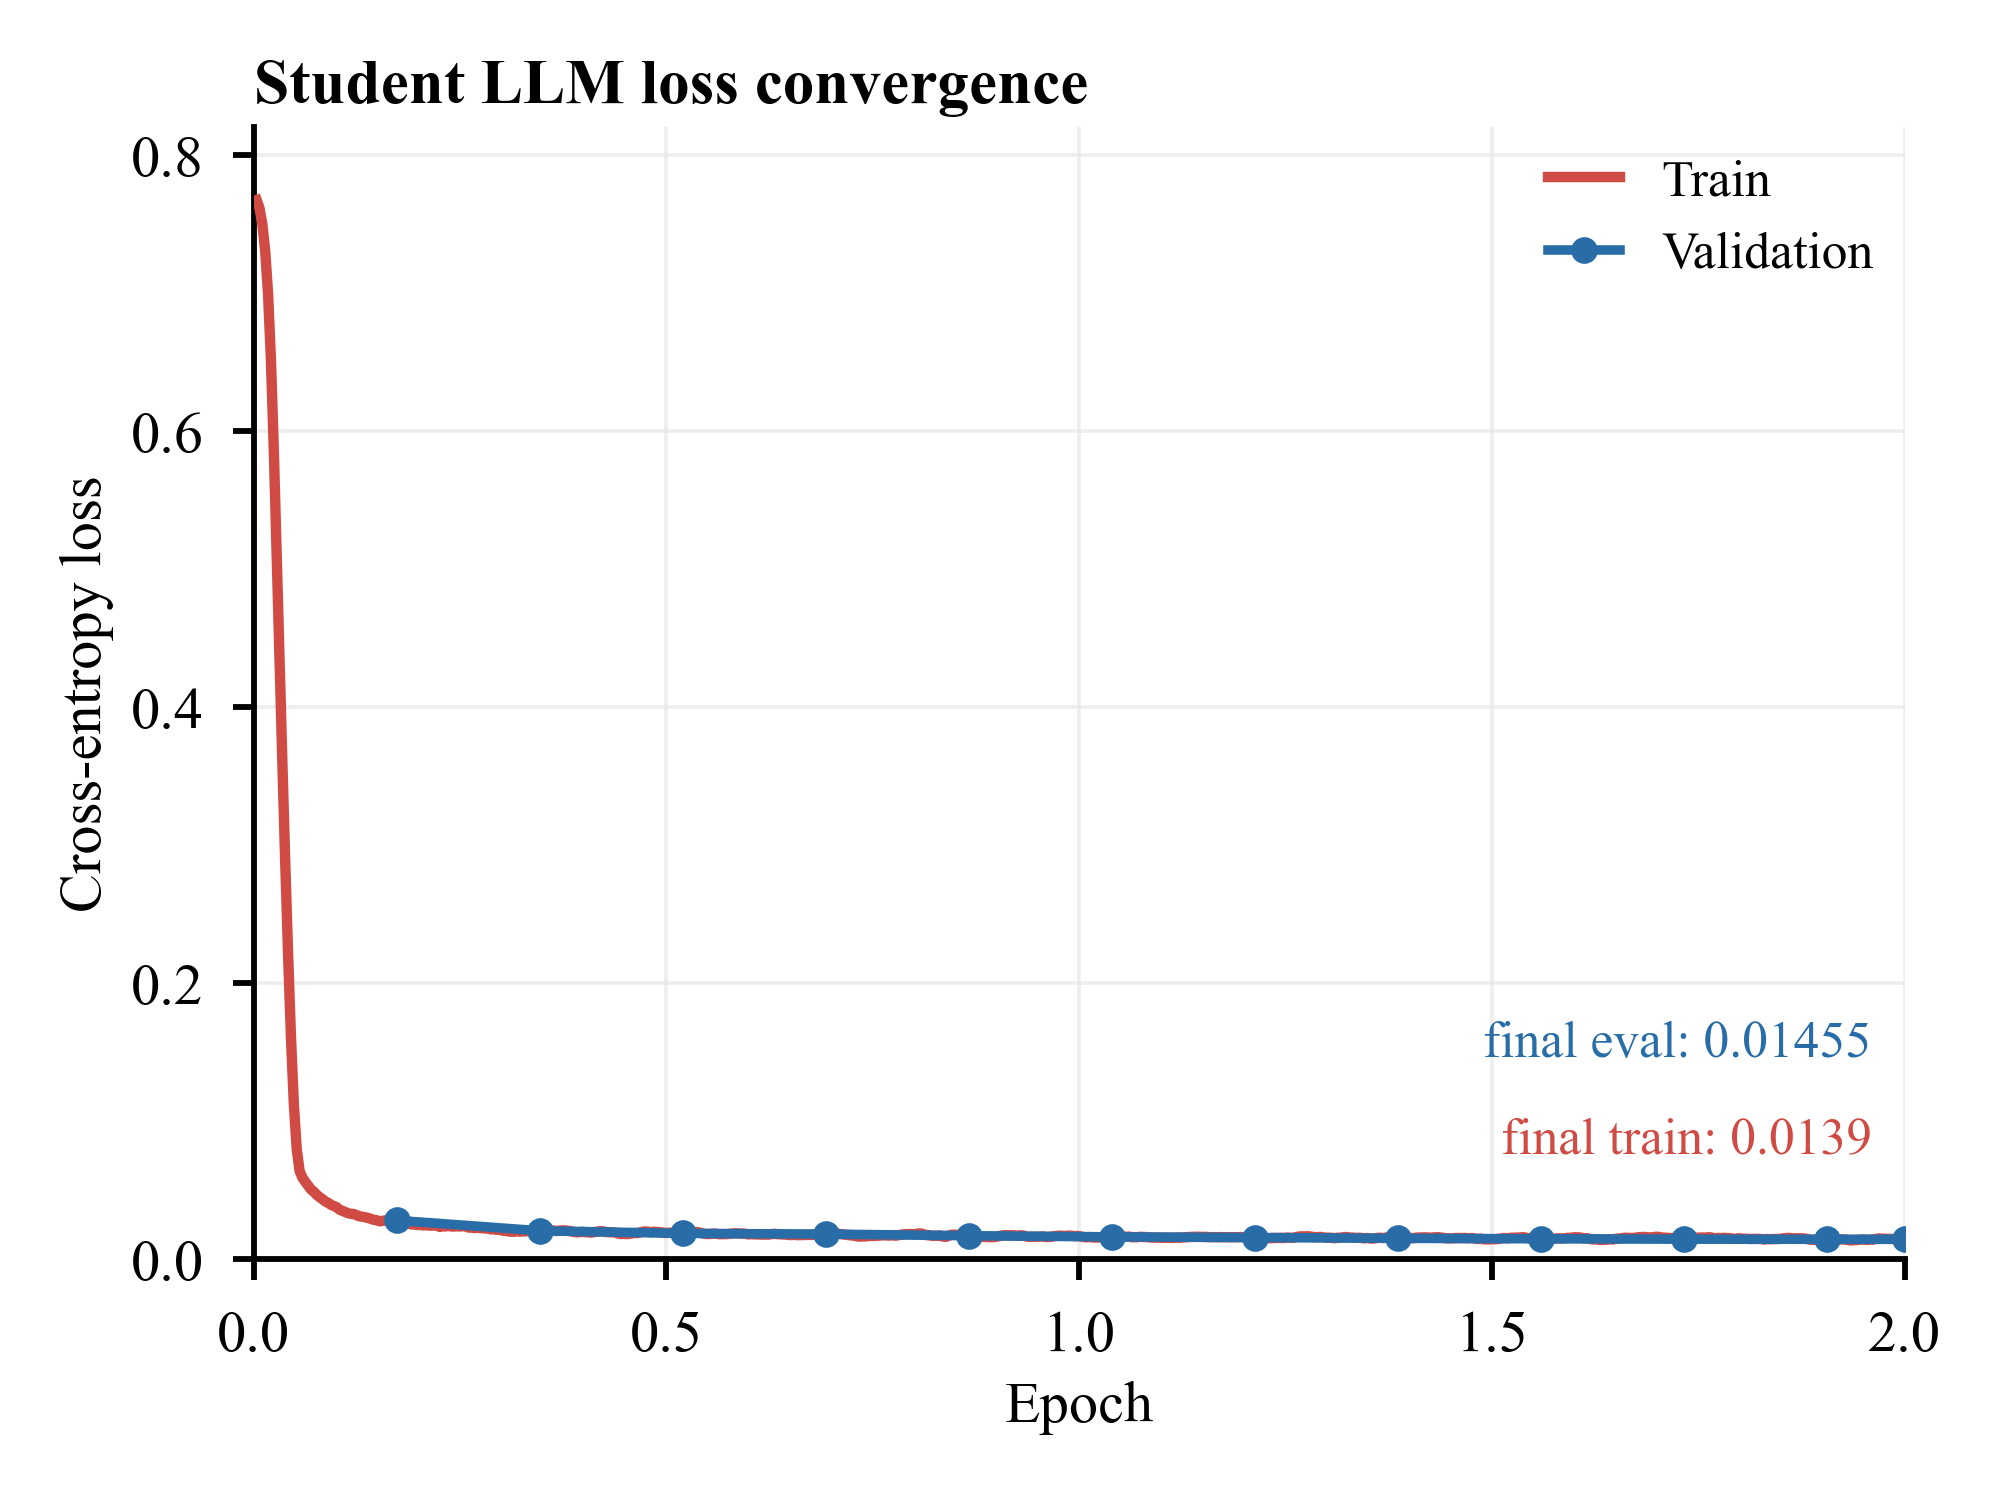
\includegraphics[width=\textwidth]{Picture/fig_llm_training_loss_convergence.png}
\par\vspace{2pt}
\noindent{\small\textbf{Fig. 1.} Student LLM training-loss convergence. The curve reports the supervised fine-tuning loss recorded during LoRA adaptation on the filtered semantic dataset; the vertical axis gives the absolute loss scale used to assess convergence stability.}

\clearpage
\section*{Appendix H: Evaluation Metrics}
\noindent All six metrics are computed from the logged state, action, and clearance histories over each evaluation episode.
\begin{enumerate}
\item \textbf{Path efficiency} (\%):
$\mathrm{PE}=\frac{L_{\mathrm{route}}}{L_{\mathrm{traveled}}}\times 100$,
where $L_{\mathrm{route}}$ is the length of the nominal route and
$L_{\mathrm{traveled}}=\sum_t\|\mathbf p_{t+1}-\mathbf p_t\|_2$ is the traveled distance.
\item \textbf{Minimum clearance} (m):
$\mathrm{MC}=\min_t\min_i d_{\mathrm{obs},i}(\mathbf p_t)$, the minimum distance to the nearest obstacle over all control instants of the episode.
\item \textbf{Risk-time ratio} (\%):
$\mathrm{RTR}=\frac{1}{T}\sum_t \mathbf 1\{\mathrm{MC}_t < d_{\mathrm{risk}}\}\times 100$,
the fraction of control instants at which the minimum clearance falls below the risk distance $d_{\mathrm{risk}}=2.25~\mathrm{m}$ (the conservative stopping-distance estimate of the platform at the evaluated operating speed).
\item \textbf{Action energy}:
$\mathrm{AE}=\sum_{t=1}^{T} \|\mathbf a_t\|_2^2$, the episode-cumulative squared action magnitude (total normalized control effort); per-step values lie in $[0,5]$. Episodes on the evaluated routes share nearly equal durations (Table~II of the main text, path length), so cumulative values are directly comparable.
\item \textbf{Action smoothness}:
$\mathrm{AS}=\frac{1}{T}\sum_t \|\mathbf a_t-\mathbf a_{t-1}\|_2$, the mean norm of consecutive action differences.
\item \textbf{Path length} (m):
$L_{\mathrm{traveled}}=\sum_t\|\mathbf p_{t+1}-\mathbf p_t\|_2$, the total traveled distance.
\end{enumerate}

\end{document}




